\begin{figure}[t]
    \centering
    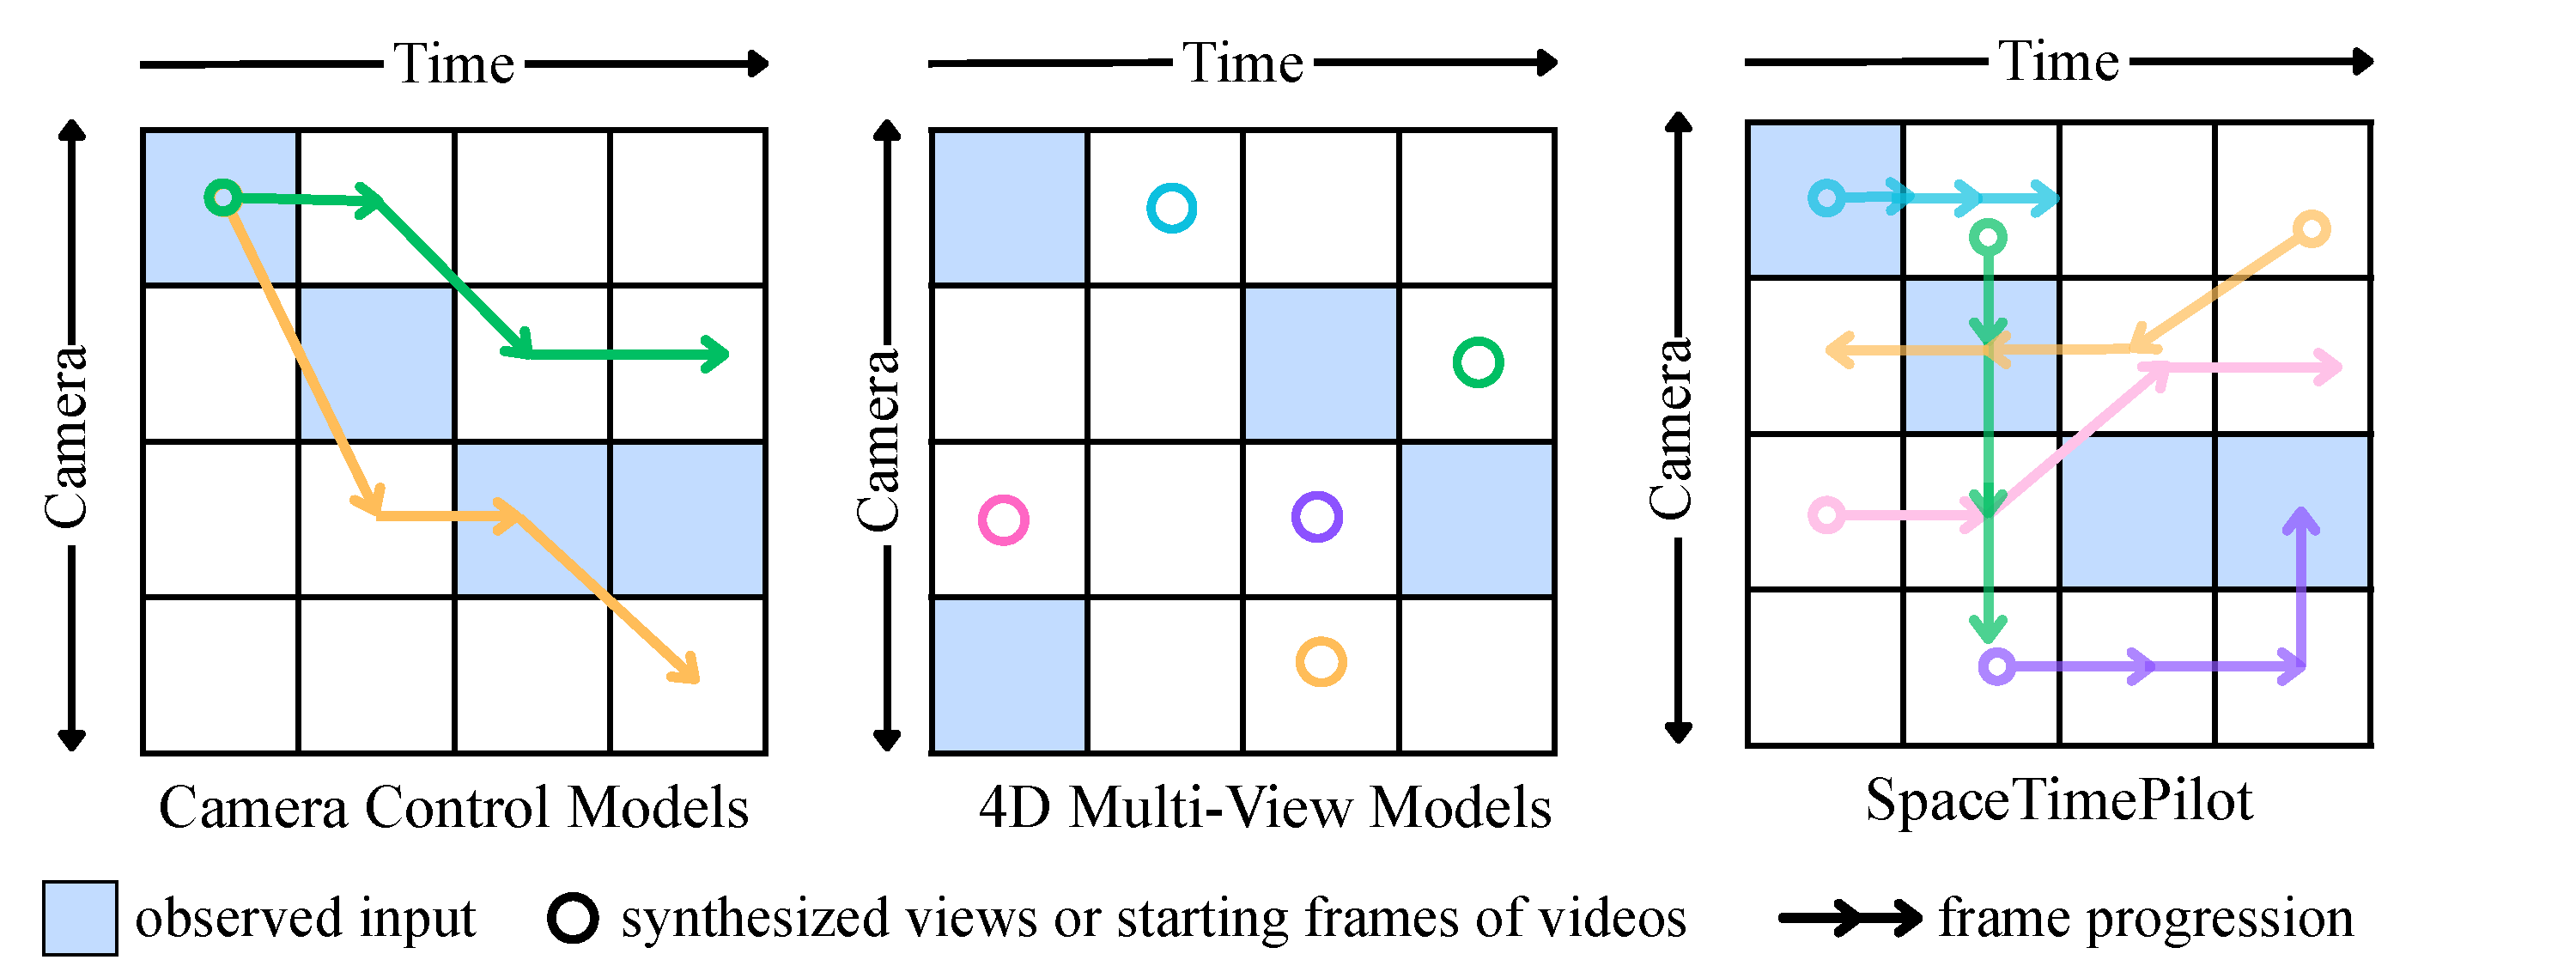
\includegraphics[width=\linewidth]{figures/src_files/high-level-concept.pdf}

\caption{\textbf{Space–time controllability across methods.}
Blue cells denote the input video/views, while arrows and dots indicate generated continuous videos or sparse frames. 
Camera-control V2V models~\cite{Bai2025, vanhoorick2024gcd} modify only the camera trajectory while keeping time strictly monotonic. 
4D multi-view models~\cite{Wu2024, liang2024diffusion4d} synthesize discrete sparse views conditioned on space and time, but do not generate continuous video sequences. 
\textit{SpaceTimePilot} enables free movement along both the camera and time axes with full control over direction and speed, supporting bullet-time, slow-motion, reverse playback, and mixed space–time trajectories.}

    \label{fig:high_level}
    \vspace{-3mm}
\end{figure}
